
Childhood is mostly spent in Type I algebra.  Learn to count. Assign 
counts the usual names $0,1,2,\ldots$.  Learn to add and multiply, and begin 
to solve questions.  Hints of new numbers show up when told to find distances of
length $\sqrt{2}$, or we learn about imaginary numbers and $\pi$.  The shift to $\pi$
signals the shift to type II because $\pi$ is such a fiddly number that it
makes sense to leave it alone moving it round solely by rules of algebra until
the end when we might replace with with 3.14 or a better approximation. For
practical purposes $\pi$ is the first quantity used as a variable. 

High school algebra is nearly all type II, and mostly following al
Khwarizmi's \emph{al Jabr}---the method of balancing parts, which today is
called Algebra.  Move over Euclid, al Khwarizmi's method made people money,
settled land disputes, calculated grain totals and arguably did more to make
math a necessity for average people than any other source. His name has passed
down to modern life as the word \emph{algorithm}. At this stage students are
told  that polynomials of degree $d$ have $d$ complex roots.  Perhaps because
some non-algebraist call this fact ``the fundamental theorem of algebra'' (it's
not) this seems a good place to leave algebra for calculus or leave math for
good.  Most people never reach a type 3 problem.

You are one of the few who have heard of type 3 algebra.
You have seen the solving linear equations gives you back often infinitely many 
answers and you don't have time nor the interest to write down infinitely many answers.
You know that this can be done with a basis.  The next example is even more 
greedy.  Why write down $d$ roots to a $d$ degree polynomial?!  Instead, you 
want to write down one solution and sprinkle in some pattern to explain how you 
might find all the others.  Think back to 
$x=\frac{-b\pm \sqrt{b^2-4ac}}{2a}$ solving $ax^2+bx+c=0$ (with $a\neq 0$).
That `$\pm$' trick saved you thinking of two roots.  Ever solved $x^6-1=0$ by 
using $x=e^{(2\pi i/6) t}$ thinking of rotating around by 60 degrees?  
These relationships turned out to have a name (groups) and were the first type 3 
algebra.

This is where the heavy weights got
involved: Lagrange made a formula for quartic polynomials from a primitive
concept of groups but he got distracted by a fluke concerning symmetric polynomials 
and missed out on the eventual full solution by Galois.
Gauss showed that construction by ruler and compass produces only numbers 
that are iterated applications of square-roots by observing what in today's 
language would say that the group of relations is nilpotent. 
Abel found a specific obstacle with $x^5-x+1=0$ by showing that if its relations 
were to be solvable they would create contradictions with facts from calculus,
the first proof that not all polynomials are solvable by radicals.  
Galois characterizes all such polynomials by describing what their type 3
algebra would look like.  Both men died tragically and without their work being 
understood until after their young deaths.

Here I should settle a confusion in the subject.  Abel and Galois did 
not show that the quintic has no solutions!  That would fly in the 
face of  Gauss' ``fundamental theorem 
of algebra'' (a 5th degree polynomial has 5 complex roots).  
What Abel and Galois proved is that roots of these polynomials where not 
of the form hinted at by the solutions for 1,2,3 and 4th degree polynomials.
Take for example al Khwarizmi's quadratic formula gives roots of the form 
$\frac{-b}{2a}\pm \frac{1}{2a}\sqrt{b^2-4ac}$, where $a,b,c$ are numbers we 
already created.  Cardano's cubic formula goes a step further.  Given 
numbers $a,\ldots, g$ already created, then solutions to the cubic can 
be made in the following form.
\[
    a+b\sqrt{c}+d\sqrt[3]{e+f\sqrt{g}}.
\]
Lagrange's quartic formula gives solutions now involving rational 
linear combinations of fourth roots.  When a number is a linear combination 
of $n$-th roots of iteratively created numbers then we say that number 
is \emph{radical}.  That the quintic is not solvable by radicals just means 
that to factor quintics and higher students need to go back to a type 1 problem:
invent new constructions of numbers. In fact, history had already done this 
for degrees 2,3.  For example, if $b^2-4ac<0$ then the solutions may be written as
\begin{align*}
    x & = \sqrt{\frac{c}{a}}\cos\theta \pm \sqrt{\frac{c}{a}}\sin\theta
    & 
    \theta & = \cos^{-1}\frac{-b}{2\sqrt{ac}}
\end{align*}
The cubic equations can likewise be solved with trigonometry.  So Abel and Galois 
point the way to revisiting how we build numbers and finding new methods.  That is,
the outcome of type 3 algebra was a need to build new type 1 algebra.

This feedback look has been hard at work for more than a century.  These new
type 1 problems lead to rings and modules.  That lead to algorithms and
representation theory to solve type 2 problems with those numbers.  Those
solutions generated new relations, more groups (type 3), but also new type 1
algebras (Clifford, Lie, Hecke, and Hopf to name a few). The iteration continues. 

As a final remark, we should settle one last potential confusion.
The fundamental theorem of algebra already told us the shape of roots,
i.e.\ complex numbers.  Why not stop here?  Answer this yourself: 
what are the roots of  $x^2=2$?  If you thought $x=\pm\sqrt{2}$ and not $x\approx \pm 1.41$ then you 
appreciate the difference.  By prescribing $x=\pm \sqrt{2}$ we both solve nothing 
(its just notation) and everything (this solution truly works).  This gets a 
a philosophical position that numbers are made up to mean what they can do. 
Real numbers are made up to mean that finite patterns that stay close together 
(Cauchy sequences) can in fact be considered as numbers (they converge to themselves,
which means nothing but lets there be real numbers).

Radical numbers like $\sqrt{2}$ are another form of invention, a number that when 
squared is $2$.  It is freeing to think this way because we can make such numbers 
precisely with ease.  For example $\begin{bmatrix} 0 & 2\\ 1 & 0\end{bmatrix}$
squares to $\begin{bmatrix} 2 & 0 \\ 0 & 2 \end{bmatrix}$ which gives precise 
calculations.  But for some situations precision wont be important and we can 
use the approximation $1.41^2\approx 2$.  Algebra therefore sees the matrix and the decimal 
examples of $\sqrt{2}$ as interchangeable. 
To algebra, $\sqrt{2}$ is a property, not so much a number.  Because of this 
we can imagine many more creative algorithms to work with these numbers.

For the purposes of solving it is important to have both 
but exact and approximate solutions.
To expose this difference 
look no further than finding the eigenvalues of a matrix.
\begin{align*}
    \begin{bmatrix}
        -9 & 7 & -12 & 6\\
        -3 & 5 & -4 & 6\\
        7 & -5 & 8 & -2\\
        2 & -2 & 4 & -4
    \end{bmatrix}
\end{align*}
With 64 bit floating points in Julia, my computer printed out 
\begin{lstlisting}
    julia> eigvals([-9 7 -12 6; -3 5 -4 6; 7 -5 8 -2; 2 -2 4 -4])
    4-element Vector{ComplexF64}:
     -0.0005295477729425071 - 0.0005295190134323146im
     -0.0005295477729425071 + 0.0005295190134323146im
      0.0005295477729438736 - 0.0005295765047025466im
      0.0005295477729438736 + 0.0005295765047025466im   
\end{lstlisting}
But actually this matrix has a single eigenvector $0$ and is not diagonalizable 
but instead it is conjugate to a nilpotent matrix:
\begin{align*}
    \begin{bmatrix}
        -9 & 7 & -12 & 6\\
        -3 & 5 & -4 & 6\\
        7 & -5 & 8 & -2\\
        2 & -2 & 4 & -4
    \end{bmatrix}
    & =
    \begin{bmatrix}
        1 & 2 &  1 & 2\\
       -1 & 2 & -1 & 2\\
         0 & 1 &  1 & 0\\
         1 & 0 &  1 &  1
   \end{bmatrix}^{-1}
   \begin{bmatrix}
        0 & 4 & 0 & 0\\
        0 & 0 & 4 & 0\\
        0 & 0 & 0 & 4\\
        0 & 0 & 0 & 0
    \end{bmatrix}
    \begin{bmatrix}
         1 & 2 &  1 & 2\\
        -1 & 2 & -1 & 2\\
          0 & 1 &  1 & 0\\
          1 & 0 &  1 &  1
    \end{bmatrix}
\end{align*}
Solutions to equations are not stable under approximations.




\section{Everything is variable}


and how expanding a solution leads to symmetries (symmetric 
polynomials by today's verbage).
\begin{align*}
    \begin{array}{|c|cc|}
        \hline
        \times & x & -b \\
        \hline
        x & x^2 & {\color{blue} -bx}\\
        -a & {\color{blue} -ax} & {\color{red} ab} \\
    \hline
    \end{array}
    & \leadsto (x-a)(x-b)=x^2{\color{blue} -(a+b)x}{\color{red}+ab}
\end{align*}
We can flip the square along the diagonal like the transpose of a matrix 
and get the same product.  Thus a symmetry that moves the roots leave the 
resulting polynomial unchanged.  For cubics we get symmetries on a cube.
\begin{center}
    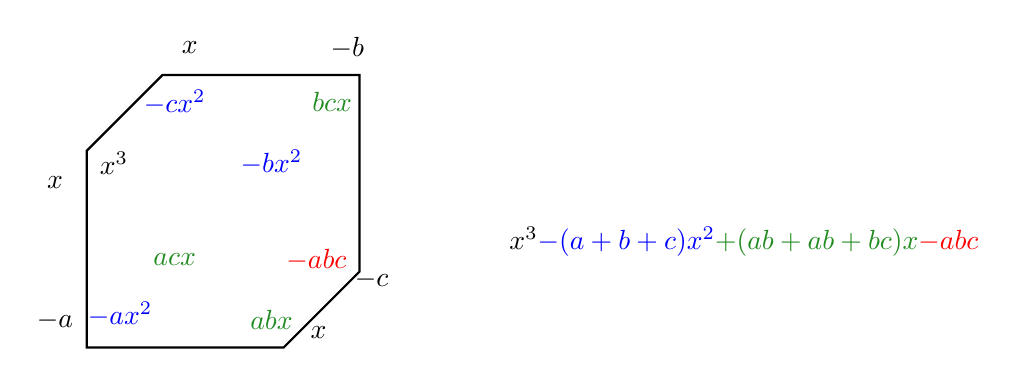
\begin{tikzpicture}
        \draw[thick] (-0.25,0.25,0.25)
            -- ++ (0,0,-2.5)
            -- ++ (2.5,0,0)
            -- ++ (0,-2.5,0)
            -- ++ (0,0,2.5)
            -- ++ (-2.5,0,0)
            -- cycle;
        \node (xx1) at (-0.75,-.25,0) {$x$};
        \node (xx2) at (0,0.5,-2.5) {$x$};
        \node (xx3) at (2.5,-2.25,-0.25) {$x$};
        \node (a) at (-0.75,-2,0) {$-a$};
        \node (b) at (2,0.5,-2.5) {$-b$};
        \node (c) at (2.5,-2.25,-2) {$-c$};

        \node (x3) at (0,0,0) {$x^3$};
        \node[blue] (ax2) at (0,-2,-0.2) {$-ax^2$};
        \node[blue] (bx2) at (2,0,0) {$-bx^2$};
        \node[blue] (cx2) at (0,0,-2) {$-cx^2$};
        \node[ForestGreen] (abx) at (2,-2,0) {$abx$};
        \node[ForestGreen] (acx) at (0,-2,-2) {$acx$};
        \node[ForestGreen] (bcx) at (2,0,-2) {$bcx$};
        \node[red] (abc) at (1.8,-2,-2) {$-abc$};

        \node at (8,-1,0) {$x^3{\color{blue}-(a+b+c)x^2}{\color{ForestGreen}+(ab+ab+bc)x}{\color{red}-abc}$};
    \end{tikzpicture}
\end{center}
Notice you can rotate or swap the three adjacent faces (permuting the three roots around) 
without interfering in the equation.  4th degree?  Explore symmetries on a hypercube.
\begin{center}
    \begin{tikzpicture}
        \draw[thick] (-4,0.5,0.5)
        -- ++ (0,0,-4.5)
        -- ++ (6.75,0,0)
        -- ++ (0,-3,0)
        -- ++ (0,0,4.5)
        -- ++ (-6.75,0,0)
        -- cycle;
        \node (xx4) at (-2,-3,0.5) {$x$};
        \node (d) at (2,-3,0.5) {$-d$};
        \node at (-2,0) {\begin{tikzpicture}
        \draw[thick] (-0.25,0.25,0.25)
            -- ++ (0,0,-2.5)
            -- ++ (2.5,0,0)
            -- ++ (0,-2.5,0)
            -- ++ (0,0,2.5)
            -- ++ (-2.5,0,0)
            -- cycle;
        \node (xx1) at (-0.75,-.25,0) {$x$};
        \node (xx2) at (0,0.5,-2.5) {$x$};
        % \node (xx3) at (2.5,-2.25,-0.25) {$x$};
        \node (a) at (-0.75,-2,0) {$-a$};
        \node (b) at (2,0.5,-2.5) {$-b$};
        % \node (c) at (2.5,-2.25,-2) {$-c$};

        \node (x3) at (0,0,0) {$x^4$};
        \node[blue] (ax2) at (0,-2,-0.2) {$-ax^3$};
        \node[blue] (bx2) at (2,0,0) {$-bx^3$};
        \node[blue] (cx2) at (0,0,-2) {$-cx^3$};
        \node[ForestGreen] (abx) at (2,-2,0) {$abx^2$};
        \node[ForestGreen] (acx) at (0,-2,-2) {$acx^2$};
        \node[ForestGreen] (bcx) at (2,0,-2) {$bcx^2$};
        \node[red] (abc) at (1.8,-2,-2) {$-abcx$};

        % \node at (8,-1,0) {$x^3{\color{blue}-(a+b+c)x^2}{\color{ForestGreen}+(ab+ab+bc)x}{\color{red}-abc}$};
        \end{tikzpicture}};
        \node at (2,0) {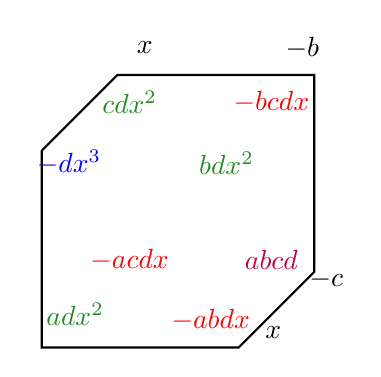
\begin{tikzpicture}
            \draw[thick] (-0.25,0.25,0.25)
                -- ++ (0,0,-2.5)
                -- ++ (2.5,0,0)
                -- ++ (0,-2.5,0)
                -- ++ (0,0,2.5)
                -- ++ (-2.5,0,0)
                -- cycle;
            % \node (xx1) at (-0.75,-.25,0) {$x$};
            \node (xx2) at (0,0.5,-2.5) {$x$};
            \node (xx3) at (2.5,-2.25,-0.25) {$x$};
            % \node (a) at (-0.75,-2,0) {$-a$};
            \node (b) at (2,0.5,-2.5) {$-b$};
            \node (c) at (2.5,-2.25,-2) {$-c$};
    
            \node[blue] (x3) at (0,0,0) {$-dx^3$};
            \node[ForestGreen] (ax2) at (0,-2,-0.2) {$adx^2$};
            \node[ForestGreen] (bx2) at (2,0,0) {$bdx^2$};
            \node[ForestGreen] (cx2) at (0,0,-2) {$cdx^2$};
            \node[red] (abx) at (1.8,-2,0) {$-abdx$};
            \node[red] (acx) at (0,-2,-2) {$-acdx$};
            \node[red] (bcx) at (1.8,0,-2) {$-bcdx$};
            \node[purple] (abc) at (1.8,-2,-2) {$abcd$};
    
            % \node at (8,-1,0) {$x^3{\color{blue}-(a+b+c)x^2}{\color{ForestGreen}+(ab+ab+bc)x}{\color{red}-abc}$};
            \end{tikzpicture}};
        \end{tikzpicture}
\end{center}
Which contracts to 
\begin{gather*}
    \begin{array}{|c|cc|}
        \hline 
         \times & x & -d \\
         \hline
        x^3 & x^4 & {\color{blue}-dx^3}\\
        -(a+b+c)x^2 & {\color{blue}-(a+b+c)x^3} & {\color{ForestGreen}(ad+bd+cd)x^2}\\
        +(ab+ac+bc)x^1 & {\color{ForestGreen}(ab+ac+bc)x^2} & {\color{red}-(abd+acd+bcd)x}\\
        -abc  & {\color{red}-abc x} & {\color{purple} abcd}\\
        \hline
    \end{array}\\
    x^4{\color{blue}-(a+b+c+d)x^3}
    {\color{ForestGreen}+(ab+ac+ad+bc+bd+cd)x^2}
    {\color{red}-(abc+abd+bcd)x}
    {\color{purple}+abcd}.
\end{gather*}
Lagrange witnessed a fluke.  You can gather the 4 roots as linear combinations
\begin{align*}
    s_{()} & = a+b+c+d\\
    s_{(12)(34)} & = a-b+c-d\\
    s_{(13)(24)} & = a-c+b-d\\
    s_{(14)(34)} & = a-d+c-b
\end{align*}
When solving a quartic, the term $s_{()}$ appears as the negative coefficient of 
$x^3$.  He then worked out how that because the remaining three are linear symmetric 
polynomials we can use them to write the other coefficients 
$(ab+ac+ad+bc+bd+cd)$, $(abc+abd+bcd)$, and $(abcd)$ as polynomials in 
the remaining $s$'s.  This means we have a single cubic polynomial which solves 
for the three missing numbers.  Having solved for all three $s$'s we use 
linear algebra to solve for the roots.
\begin{align*}
    \begin{bmatrix} 
        1 & 1 & 1 & 1\\
        1 & -1 & 1 & -1\\
        1 & 1 & -1 & -1\\
        1 & -1 & -1 & 1
    \end{bmatrix}
    \begin{bmatrix}
        a\\ b\\ c\\ d 
    \end{bmatrix}
    & = 
    \begin{bmatrix}
        s_{()}\\
        s_{(12)(34)}\\
        s_{(13)(24)}\\
        s_{(14)(32)}
    \end{bmatrix}
\end{align*}


